\documentclass[10pt]{article}
\usepackage{icmlko}

\icmlmeta{IP 파운데이션 월드모델}{204}{풀은 업어 주고 눌러 준다}{노트 203이 ``풀링 항을 무엇이 예측하나''를 남겼다. 후보 넷이 다 실패하고 뜻밖의 것이 나왔다 --- 풀링을 제일 잘 예측하는 것은 혼자였고, 그 관계에 기울기가 있다}

\begin{document}

\twocolumn[
\icmlheader

\begin{abstract}
노트 203이 도메인 성질 셋으로 ``혼자 학습한 $\rho$''를 $+$0.750 예측했는데
``풀에서 뺄까''(격차 $=$ 혼자 $-$ 풀링)는 $+$0.143 으로 못 맞혔고, 남은 길로
``풀링 항을 따로 예측하라''를 적었다. 후보 넷을 댔다 --- 나머지와의 계수
코사인(가중 · 평균) · 나머지 도메인의 총 학습 행 · 내 학습 몫.
\textbf{넷 다 실패한다}($|\rho| \le 0.32$). 대신 뜻밖의 것이 1위다 ---
\textbf{풀링을 제일 잘 예측하는 것은 혼자다}($+$0.750). 회귀하면
\[\text{풀링} = 0.127 + 0.688 \times \text{혼자}, \quad R^2 = 0.733\]
\textbf{기울기가 1 보다 작다.} 풀은 약한 도메인을 절편만큼 \emph{업어 주고}
($+$0.127) 강한 도메인을 기울기만큼 \emph{눌러 준다}(0.688). 웹툰은 혼자
$+$0.090 인데 풀에서 $+$0.248 을 받고, 모바일은 혼자 $+$0.514 인데 풀에서
$+$0.438 밖에 못 받는다. 두 선이 만나는 곳이 \textbf{손익분기 혼자
$\rho{=}0.407$} 이다. 그 규칙으로 판정하면 일곱 중 넷을 맞히는데,
\textbf{격차가 검출 한계(0.04)를 넘는 셋 --- 게임 · 모바일 · 웹툰 --- 은
3/3 이다.} 틀린 셋은 전부 $|$격차$| < 0.04$ 로 노트 152의 짝 반폭 안이다.
회귀선에서 벗어난 잔차는 나머지와의 코사인과 $+$0.36(스피어만) ·
$+$0.44(피어슨)로 방향은 맞지만 약하다 --- \textbf{닮음이 미세 조정은 하고
결정은 안 한다}(노트 197의 $-$0.25 와 이어진다). 그래서 이 갈래의 답은
\textbf{``격차를 예측하려 하지 말고 혼자 $\rho$ 를 재라''}이다. 노트 197의
이분 규칙이 하던 일이 정확히 그것이었고, 이제 그 손익분기가 어디인지 안다.
\end{abstract}
]

\begin{figure*}[t]
\centering
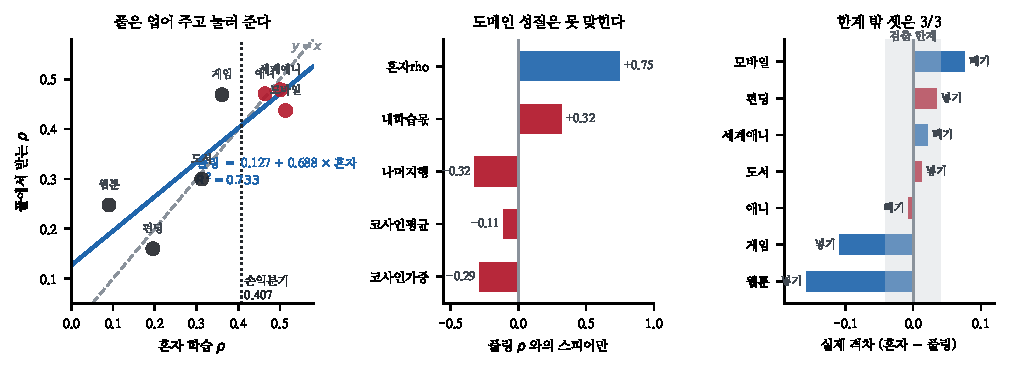
\includegraphics[width=\textwidth]{figs/carry2.pdf}
\caption{왼쪽 --- 풀은 업어 주고 눌러 준다. 가운데 --- 도메인 성질은 못
맞힌다. 오른쪽 --- 한계 밖 셋은 3/3.}
\end{figure*}

\section{후보 넷이 다 실패한다}

\begin{table}[t]
\centering\tsize
\caption{풀링 $\rho$ 와의 스피어만.}
\begin{tabular}{lr}
\toprule
나머지와의 코사인(가중) & $-$.286 \\
나머지와의 코사인(평균) & $-$.107 \\
나머지 도메인 총 학습 행 & $-$.321 \\
내 학습 몫 & $+$.321 \\
\midrule
\textbf{혼자 $\rho$} & \textbf{$+$.750} \\
\bottomrule
\end{tabular}
\end{table}

\claimx{\textbf{``나머지와 얼마나 닮았나''가 풀링을 안 정한다}($-$0.29).
노트 203이 걸어 둔 처방인데 틀렸다 --- 그리고 부호까지 반대다.}{노트 197에서
코사인이 풀링 \emph{이득}과 $-$0.25 였는데, 혼자 항을 뺀 뒤에도 여전히
약하다. \textbf{계수가 닮았다고 풀이 잘 맞는 것이 아니다.}}

\section{풀은 압축한다}

\begin{table}[t]
\centering\tsize
\caption{풀링 $=$ 0.127 $+$ 0.688 $\times$ 혼자. $R^2{=}0.733$.}
\begin{tabular}{lrrr}
\toprule
& 혼자 & 풀링 & 격차 \\
\midrule
\textbf{모바일} & \textbf{.514} & .438 & \textbf{$+$.076} \\
세계애니 & .501 & .479 & $+$.022 \\
애니 & .464 & .471 & $-$.007 \\
\midrule
\multicolumn{4}{c}{\emph{손익분기 .407}} \\
\midrule
게임 & .361 & \textbf{.469} & \textbf{$-$.108} \\
도서 & .312 & .300 & $+$.013 \\
펀딩 & .195 & .160 & $+$.035 \\
\textbf{웹툰} & \textbf{.090} & \textbf{.248} & \textbf{$-$.158} \\
\bottomrule
\end{tabular}
\end{table}

\claimx{\textbf{기울기 0.688 이 1 보다 작다.} 풀은 약한 도메인을 절편만큼
업어 주고 강한 도메인을 기울기만큼 눌러 준다 --- 웹툰 $+$0.090 $\to$
$+$0.248, 모바일 $+$0.514 $\to$ $+$0.438.}{노트 197이 ``풀링은 닮아서가
아니라 업어 주기 때문''을 말로 세웠는데, \textbf{여기서 그것이 절편과
기울기라는 두 수로 나온다.} 업어 주는 것은 절편이고 누르는 것은 기울기다.}

\claimx{\textbf{$R^2{=}0.733$ 이다.} 도메인이 풀에서 받는 것의 4분의 3이
그 도메인이 혼자 할 수 있는 것으로 설명된다 --- 나머지 아홉이 누구인지와
거의 무관하다.}{이건 노트 203의 물음(``풀링 쪽은 나머지가 정한다'')을
정정한다 --- \textbf{나머지가 정하는 것은 4분의 1뿐이다.}}

\section{손익분기 0.407}

\begin{table}[t]
\centering\tsize
\caption{혼자 $\rho > 0.407$ 이면 빼고 아니면 넣는다.}
\begin{tabular}{lrrl}
\toprule
& 판정 & 실제 격차 & \\
\midrule
\textbf{모바일} & 빼기 & $+$.076 & \textbf{O} \\
\textbf{게임} & 넣기 & $-$.108 & \textbf{O} \\
\textbf{웹툰} & 넣기 & $-$.158 & \textbf{O} \\
\midrule
세계애니 & 빼기 & $+$.022 & O \\
애니 & 빼기 & $-$.007 & X \\
도서 & 넣기 & $+$.013 & X \\
펀딩 & 넣기 & $+$.035 & X \\
\bottomrule
\end{tabular}
\end{table}

\claimx{\textbf{격차가 검출 한계를 넘는 셋은 3/3 이다.} 틀린 셋은 전부
$|$격차$| < 0.04$ 로, 노트 152가 잰 짝 반폭 안이다 --- \textbf{맞고 틀리고를
따질 크기가 아니다.}}{전체로는 4/7 인데 그 숫자는 오해를 부른다. 노트 200의
``개수로 세지 말고 무게로 세라''가 여기서도 걸린다.}

\claimx{잔차(회귀선에서 벗어난 정도)는 나머지와의 코사인과 $+$0.36 ·
$+$0.44 다 --- \textbf{닮음이 미세 조정은 하고 결정은 안 한다.} 게임이
잔차 $+$0.094 로 제일 크고 코사인도 0.649 로 제일 높다.}{그래서 게임이
손익분기 아래인데도 풀링이 예상보다 더 잘 맞는다 --- \textbf{닮음의 값어치가
있다면 거기에 있다.}}

\section{이 갈래의 답}

\claimx{\textbf{격차를 예측하려 하지 말고 혼자 $\rho$ 를 재라.} 격차는 두
상관된 양($+$0.750)의 차이라 예측이 어렵고, 혼자 $\rho$ 하나면 손익분기로
판정된다.}{\textbf{노트 197의 이분 규칙이 하던 일이 정확히 그것이다} ---
안쪽에서 혼자와 풀링을 견줘 고르는 것은 손익분기를 자료로 찾는 것과 같다.
이제 그 분기가 $+$0.407 인 줄 안다.}

\begin{table}[t]
\centering\tsize
\caption{노트 203$\sim$204 가 답한 것.}
\begin{tabular}{ll}
\toprule
혼자 할 수 있나 & 도메인 성질 셋으로 $+$0.750 \\
풀에서 얼마 받나 & 혼자로 $R^2{=}0.733$ \\
\textbf{풀에 넣을까} & \textbf{혼자 $\rho$ 를 0.407 과 견준다} \\
나머지가 정하는 몫 & 4분의 1 (잔차) \\
\bottomrule
\end{tabular}
\end{table}

\begin{table}[t]
\centering\tsize
\caption{남은 것.}
\begin{tabular}{ll}
\toprule
\textbf{손익분기} & 0.407 은 이 판 · 이 열 도메인의 값 \\
잔차 & 코사인이 $+$0.44 --- 더 나은 닮음 재기 \\
\textbf{트리} & 이 갈래 전부 능형 --- F18 은 압축이 다를 것 \\
\bottomrule
\end{tabular}
\end{table}

마지막 줄이 제일 크고 곧바로 잴 수 있다. 이 압축 관계(절편 0.127 · 기울기
0.688)는 능형에서 잰 것이다. \textbf{트리는 도메인 절편뿐 아니라 도메인으로
쪼갤 수 있으므로 덜 압축할 것이다} --- 기울기가 1 에 가까우면 풀이 누르지
않는다는 뜻이고, 그러면 챔피언에서는 도메인을 뺄 이유가 아예 없다.
\textbf{그것이 맞으면 노트 197$\sim$204 의 갈래 전체가 선형에만 해당하는
이야기가 된다.}

\end{document}
